%% 
%% Copyright 2007, 2008, 2009 Elsevier Ltd
%% 
%% This file is part of the 'Elsarticle Bundle'.
%% ---------------------------------------------
%% 
%% It may be distributed under the conditions of the LaTeX Project Public
%% License, either version 1.2 of this license or (at your option) any
%% later version.  The latest version of this license is in
%%    http://www.latex-project.org/lppl.txt
%% and version 1.2 or later is part of all distributions of LaTeX
%% version 1999/12/01 or later.
%% 
%% The list of all files belonging to the 'Elsarticle Bundle' is
%% given in the file `manifest.txt'.
%% 

%% Template article for Elsevier's document class `elsarticle'
%% with numbered style bibliographic references
%% SP 2008/03/01

\documentclass[preprint,12pt,authoryear]{elsarticle}

%% Use the option review to obtain double line spacing
%% \documentclass[authoryear,preprint,review,12pt]{elsarticle}

%% Use the options 1p,twocolumn; 3p; 3p,twocolumn; 5p; or 5p,twocolumn
%% for a journal layout:
%% \documentclass[final,1p,times]{elsarticle}
%% \documentclass[final,1p,times,twocolumn]{elsarticle}
%% \documentclass[final,3p,times]{elsarticle}
%% \documentclass[final,3p,times,twocolumn]{elsarticle}
%% \documentclass[final,5p,times]{elsarticle}
%% \documentclass[final,5p,times,twocolumn]{elsarticle}

%% For including figures, graphicx.sty has been loaded in
%% elsarticle.cls. If you prefer to use the old commands
%% please give \usepackage{epsfig}

%% The amssymb package provides various useful mathematical symbols
\usepackage{amssymb}
\usepackage{amsmath}
\usepackage{url}
%% The amsthm package provides extended theorem environments
%% \usepackage{amsthm}

%% The lineno packages adds line numbers. Start line numbering with
%% \begin{linenumbers}, end it with \end{linenumbers}. Or switch it on
%% for the whole article with \linenumbers.
\usepackage{lineno}

%% Block of code for fixing corresponding author bug 
%% in elsarticle template... Don't really understand it
\makeatletter
\def\@author#1{\g@addto@macro\elsauthors{\normalsize%
    \def\baselinestretch{1}%
    \upshape\authorsep#1\unskip\textsuperscript{%
      \ifx\@fnmark\@empty\else\unskip\sep\@fnmark\let\sep=,\fi
      \ifx\@corref\@empty\else\unskip\sep\@corref\let\sep=,\fi
      }%
    \def\authorsep{\unskip,\space}%
    \global\let\@fnmark\@empty
    \global\let\@corref\@empty  %% Added
    \global\let\sep\@empty}%
    \@eadauthor={#1}
}
\makeatother
%% End block of weird code

%% Command for bold Greek symbols
\newcommand{\mitbf}[1]{\hbox{\mathversion{bold}$#1$}}


\journal{Physics of Earth and Planetary Interiors}

\begin{document}

\begin{frontmatter}

%% Title, authors and addresses

%% use the tnoteref command within \title for footnotes;
%% use the tnotetext command for theassociated footnote;
%% use the fnref command within \author or \address for footnotes;
%% use the fntext command for theassociated footnote;
%% use the corref command within \author for corresponding author footnotes;
%% use the cortext command for theassociated footnote;
%% use the ead command for the email address,
%% and the form \ead[url] for the home page:
%% \title{Title\tnoteref{label1}}
%% \tnotetext[label1]{}
%% \author{Name\corref{cor1}\fnref{label2}}
%% \ead{email address}
%% \ead[url]{home page}
%% \fntext[label2]{}
%% \cortext[cor1]{}
%% \address{Address\fnref{label3}}
%% \fntext[label3]{}

\title{Scaling rates of true polar wander in convecting planets and moons}

%% use optional labels to link authors explicitly to addresses:
%% \author[label1,label2]{}
%% \address[label1]{}
%% \address[label2]{}

\author{Ian Rose\corref{cor1}\fnref{ref1}}
\author{Bruce Buffett\fnref{ref1}}

\fntext[ref1]{University of California, Berkeley}
\cortext[cor1]{Corresponding author, \url{ian.rose@berkeley.edu}}

\address{}

\begin{abstract}
Mass redistribution in the convecting mantle of a planet causes perturbations in its moment of inertia tensor. 
Conservation of angular momentum dictates that these perturbations change the direction of the rotation vector of the planet, a process known as true polar wander (TPW). 
Although the existence of TPW on Earth is firmly established, its rate and magnitude over geologic time scales remain controversial. 
Here we present scaling analyses and numerical simulations of TPW due to mantle convection over a range of parameter space relevant to planetary interiors. 
For simple rotating convection, we identify a set of dimensionless parameters that fully characterize true polar wander. We use these parameters to define  timescales for the growth of moment of inertia perturbations due to convection and for their relaxation due to true polar wander. 
These timescales, as well as the relative sizes of convective anomalies, control the rate and magnitude of TPW.
This analysis also clarifies the nature of so called ``inertial interchange'' TPW events, and relates them to a  broader class of events that enable large and often rapid TPW. We expect these events to have been more frequent in Earth's past.
\end{abstract}

\begin{keyword}
Rotational variations; polar wobble \sep
Paleomagnetism \sep
Models of interior structure \sep
Planetary interiors \sep
Convection currents and mantle plumes \sep
\PACS 91.10.Nj \sep 91.25.Ng \sep 91.35.Cb \sep 91.45.Bg \sep 91.45.Fj
%% keywords here, in the form: keyword \sep keyword

%% PACS codes here, in the form: \PACS code \sep code

%% MSC codes here, in the form: \MSC code \sep code
%% or \MSC[2008] code \sep code (2000 is the default)

\end{keyword}

\end{frontmatter}

\linenumbers

\section{Introduction}
\label{sec:intro}

A rotating, quasistatic body like a planetary mantle will tend to spin about the axis of its maximum moment of inertia.
Convection in a planetary mantle continuously redistributes mass, which can change the moment of inertia tensor, necessitating a change in the spin axis of the planet to conserve angular momentum, a process known as true polar wander (TPW).

TPW was first considered in detail by \citet{darwin1887influence}, and the theory has been subsequently developed by many \citep[e.g.][]{munk1960rotation, goldreich1969some, ricard1993polar}. 
Despite this, the ability of internal mass anomalies to drive large-scale TPW remains controversial. 
Paleomagnetic data have been interpreted to require up to $3^\circ-12^\circ$/Myr rates of TPW \citep{mitchell2011sutton}, but the ability of the mantle to respond at such rates has been questioned \citep{tsai2007theoretical}.

The primary uncertainties in assigning a maximum TPW rate to a convecting planet are the size of convective anomalies, which drive the rotational adjustment, and the viscosity structure of the mantle, which retards it. 
These two uncertainties are not unrelated: they are both expected to be functions of the geometric and material properties of the mantle.
As such, they do not vary independently, and first-order questions about the propensity for planets to experience TPW remain: how are rates of TPW expected to vary with the vigor of convection? 
Are other planetary bodies more or less likely than Earth to experience TPW?  And are these rates expected to vary through Earth history?

These questions suggest that an approach rooted in dimensional analysis and fluid dynamics can clarify the rates and magnitudes of TPW.
Most previous studies coupling mantle convection models to polar wander calculations have done so with prescribed density perturbations \citep[e.g.][]{greff2004upwelling}, or prescribed moment of inertia variations \citep[e.g.][]{tsai2007theoretical, creveling2012mechanisms}. 
\citet{richards1999polar} coupled thermal convection models to a polar wander model, but did not address in detail the scaling relationships between the two.

Herein we perform a scaling analysis of rates of TPW for a minimal system of a rotating, convecting mantle. We identify a set of dimensionless parameters that fully characterize TPW and use numerical simulations to quantify the expected dependence on these parameters. Finally, we use the scaling results to make predictions about TPW over Earth's history and for other planetary bodies. 

\section{Rotational dynamics}
\label{sec:rotational_dynamics}

\subsection{The Liouville equation}
\label{sec:liouville}
Conservation of angular momentum for a torque-free system in a rotating reference frame requires

\begin{equation}
\frac{d \mathbf{H}}{dt} + \mitbf{\Omega} \times \mathbf{H} = 0
\label{eq:euler}
\end{equation}
where $\mathbf{H} = \mathbf{I} \cdot \mitbf{\Omega}$ is the angular momentum vector, $\mathbf{I}$ is the moment of inertia tensor, and $\mitbf{\Omega}$ is the angular velocity vector.
On a dynamic planet $\mathbf{I}$ is a function of time, so $\mitbf{\Omega}$ must also vary with time to conserve angular momentum.
In this case, Equation~\eqref{eq:euler} is often called the Liouville equation \citep[e.g.][]{munk1960rotation}.
For a slowly convecting fluid, such as a planetary mantle, the inertial term $\partial \mathbf{H} / \partial t$ is negligible, so we may solve the simplified quasistatic equations
\begin{equation}
\mitbf{\Omega } (t)\times ( \mathbf{I}(t) \cdot \mitbf{\Omega }(t) ) = 0.
\label{eq:quasistatic_liouville}
\end{equation}
Equation~\eqref{eq:quasistatic_liouville} indicates that $\mitbf{\Omega}$ and $\mathbf{H}$ are parallel, so a solution for $\mitbf{\Omega}(t)$ is equivalent to solving an eigenvalue problem for the principal values of $\mathbf{I}(t)$;  the eigenvectors define the principal axes and the eigenvalues correspond to the principal moments of inertia. The rotation axis is expected to align with the axis for the largest moment.  
In practice, this eigenvalue approach has been often used in previous studies for computing the spin axis of a planet \citep[e.g.][]{steinberger1997changes, roberts2007cause}.
The moment of inertia tensor in Equation~\eqref{eq:quasistatic_liouville} includes all contributions to the mass structure
of the planet, including the spherically symmetric mass distribution, rotational deformation, deformation due to self gravity, internal and surface density anomalies, and the associated surface deflections.
Here we are interested in those contributions that arise from mantle convection.


The moment of inertia tensor is commonly separated into three parts for mantle convection problems \citep{sabadini1981pleistocene, spada1992excitation}:
\begin{equation}
I_{ij}(t) = I_0 \delta_{ij} + J_{ij}(t) + E_{ij}(t)
\label{eq:separation}
\end{equation}
where $I_0$ is the spherically symmetric reference moment, $J_{ij}$ is the contribution due to rotational deformation, and $E_{ij}$ is the contribution due to internal density anomalies, as well as the surface deflections caused by them.
If we plug this decomposition into Equation~\eqref{eq:quasistatic_liouville} the spherically symmetric part $I_0 \delta_{ij}$ drops out, and we are left with
\begin{equation}
\mathbf{\Omega} \times (\mathbf{J} \cdot \mitbf{\Omega}) = -\mitbf{\Omega} \times ( \mathbf{E} \cdot \mitbf{\Omega} ).
\label{eq:disequilibrium}
\end{equation}
This form of the quasistatic Liouville equation makes clear that the polar wander problem represents a balance between the mismatches
of the convective part of the moment of inertia ($\mathbf{E}$) and the rotational deformation part of the moment of inertia ($\mathbf{J}$).
Our goal is to characterize this balance from a perspective of scaling and fluid dynamics.

\subsection{A note on reference frames}
\label{sec:reference_frames}
True polar wander can be described in different reference frames, and this choice is fundamentally an arbitrary one.
However, certain aspects of the physics can be made much simpler by an appropriate choice of the reference frame.
In our treatment of TPW, we will refer to three different reference frames.  First, there is the inertial, non-rotating frame corresponding to spatial coordinates that are fixed in time.
 Second, there is the body-fixed (or geographic) frame.
By definition, the rotation of the body-fixed frame relative to the inertial frame is specified by $\mitbf{\Omega}$.
A terrestrial no-net-rotation or hotspot reference frame are common choices for the body-fixed frame.
Treatments of gravitational or rotational deformation of a planet are most naturally expressed in the body-fixed frame,
as described in Section~\ref{sec:rotational_deformation}.
 Finally, there is the frame described by the principal axes of convective part of the moment of inertia $\mathbf{E}$,
which we will refer to as the ``$\mathbf{E}$-frame.'' 
Redistribution of mantle mass anomalies due to convection changes the principal axes of $\mathbf{E}$, 
causing the $\mathbf{E}$-frame to slowly rotate with respect to the geographic frame. 


\subsection{Rotational deformation}
\label{sec:rotational_deformation}

Rotational deformation in an elastic body is traditionally related to the degree-two part of the 
centrifugal potential using a Love-number formalism. When the perturbation in gravitational
potential is related to the moments of inertia using MacCullagh's formula  \citep{munk1960rotation}, we find:
\begin{equation}
J_{ij} = \frac{k a^5}{3 G} \left( \Omega_i \Omega_j - \frac{1}{3} \Omega_q \Omega_q \delta_{ij} \right)
\label{eq:elastic_deformation}
\end{equation}
where $k$ is an elastic Love number, $a$ is the semimajor axis of the planet, and $G$ is the gravitational constant. Both $\Omega_i$ and
$J_{ij}$ are defined in the body-fixed frame. An extension to  viscoelastic rheology is permitted by the viscoelastic correspondence principle \citep[e.g.][]{peltier1974impulse}:
\begin{equation}
J_{ij} = \frac{k(t) a^5}{3 G} * \left( \Omega_i \Omega_j - \frac{1}{3} \Omega_q \Omega_q \delta_{ij} \right)
\label{eq:viscoelastic_deformation}
\end{equation}
where $k$ is now a time-dependent viscoelastic Love number which is convolved with the time-dependent rotation vector.

The infinite-time limit of Equation~\eqref{eq:viscoelastic_deformation} for a 
constant rotation vector around the $z$-axis implies
\begin{equation}
\begin{aligned}
J_{zz} = C = &\frac{2}{3} \frac{k_f a^5 \Omega^2}{3 G} \\
J_{xx} = J_{yy} = A = -&\frac{1}{3} \frac{k_f a^5 \Omega^2}{3 G} \\
\end{aligned}
\end{equation}
where $C$ and $A$ are the polar and equatorial moments of inertia, respectively, 
and $k_f$ is the fluid limit of $k$. 
We can solve for $k_f$ in terms of $C-A$:
\begin{equation}
k_f = \frac{3 G (C-A)}{\Omega^2 a^5}.
\label{eq:fluid_love}
\end{equation}
This infinite-time limit  ensures that the left-hand side of Equation (4) vanishes. It follows that the contribution from the convective perturbation $E_{ij}$ also vanishes, so no further TPW is permitted.

\citet{ricard1993polar} obtain an approximation to Equation~\eqref{eq:viscoelastic_deformation} which retains its long-time behavior by entering the Laplace domain and truncating a Taylor series for $k(s)$ to first order.  
This introduces a new parameter, $\tau_R$, which can be seen as a weighted relaxation time for the system.  
This simple approximation in the Laplace domain allows for an analytical transformation back into the time domain. Neglecting second order terms in $\dot{\Omega}$ we find:
\begin{equation}
J_{ij} = \frac{k_f a^5}{3 G} \left( \Omega_i \Omega_j - \frac{1}{3} \Omega_q \Omega_q \delta_{ij} \right) -
 \frac{k_f a^5 \tau_R}{3G} \left(\dot{\Omega}_i \Omega_j + \Omega_i \dot{\Omega}_j - \frac{2}{3} \Omega_q \dot{\Omega}_q \delta_{ij} \right).
\label{eq:rotational_deformation}
\end{equation}
The two terms of this equation have simple interpretations.  
The first term corresponds to the fluid limit of rotational deformation (in the absence of any long-term elastic strength).  
The second term represents the lag in the moment of inertia due to the viscous adjustment of the rotational bulge, where $\tau_R$ is the characteristic time constant for this adjustment.
Since the first term represents the hydrostatic limit of rotational deformation, it automatically satisfies Equation~\eqref{eq:quasistatic_liouville}, and hence does not contribute to the polar wander problem.

\subsection{The convective moment of inertia}
\label{sec:convective_moment}

The term on the right-hand side of Equation~\eqref{eq:disequilibrium} represents the moment of inertia due to internal density anomalies as well as the surface deflections due to them.
Both of these contributions may also be parameterized using a viscoelastic Love number approach:
\begin{equation} 
\mathbf{E} = \left[ \delta(t) + k^L(t) \right] * \mathbf{C}
\end{equation}
where $k^L$ is an internal loading Love number representing the surface deflection due to density anomalies, 
and $C_{ij}$ is the moment of inertia due solely to the internal load.
When the timescale of the surface response is short compared to the true polar wander timescale, it is reasonable to  use the fluid limit geoid kernels \citep[e.g.][]{richards1984geoid}:  
\begin{equation}
E_{ij} = (1+k^L_f) C_{ij}.
\end{equation}
An alternative to the Love number formalism is to calculate surface deflections directly using mantle convection simulations with a true free surface boundary condition.
A recent implementation of a free surface boundary condition in the CIG-sponsored mantle convection software \texttt{ASPECT} \citep{rose2016free}
permits more general treatments of mantle rheology.

\subsection{Rate of true polar wander}
\label{sec:tpw_rate}

We are in a position to address the rates of true polar wander for a given convective moment $\mathbf{E}$.
A considerable simplification occurs if we neglect secular changes in the rotation rate, and just consider changes in direction of the pole ($d \Omega^2 / dt = 2 {\Omega_i} \dot{ \Omega}_i = 0$)
Substituting Equation~\eqref{eq:rotational_deformation} into Equation~\eqref{eq:disequilibrium} we find
\begin{equation}
\frac{k_f a^5 \tau_R \Omega^2}{3G}\mitbf{\Omega} \times \dot{\mitbf{\Omega} } = \mitbf{\Omega} \times \left( \mathbf{E} \cdot \mitbf{\Omega} \right).
\label{eq:liouville}
\end{equation}
Introducing a unit vector $\mitbf{\omega} = \mitbf{\Omega}/\|\mitbf{\Omega} \|$ and using Equation~\eqref{eq:fluid_love} for $k_f$,  we may solve this equation for $\dot{\mitbf{\omega}}$:
\begin{equation}
 \dot{\mitbf{\omega}}  = \frac{1}{(C-A)\tau_R} \left[ \mathbf{E} \cdot \mitbf{\omega} - \left( \mitbf{\omega} \cdot \mathbf{E} \cdot \mitbf{\omega}  \right) \mitbf{\omega} \right].
\label{eq:liouville_ode}
\end{equation}
In order to evaluate $\dot{\mitbf{\omega}}$ we require knowledge of both $\mathbf{E}$ and $\mitbf{\omega}$ in the geographic frame (i.e. the frame used to derive Equation (13)). The same frame is also used to measure TPW, but the expressions on the right-hand-side of Equation (13) are more naturally evaluated in the reference frame of the principal axes of $\mathbf{E}$.
We can avoid the need to reconcile these two frames by confining our attention to the rate of TPW because scalar quantities are invariant under coordinate rotations. (We denoted  the rate of wander by 
 $\dot{W} = \vert \dot{\mitbf{\omega}} \vert$) .
Evaluating the scalar product $\dot{W}^2 = \dot{\mitbf{\omega}} \cdot \dot{\mitbf{\omega}}$ gives
\begin{equation}
\dot{W}^2 = \dot{\mitbf{\omega}}^2 = \frac{1}{(C-A)^2 \tau_R^2} \left[ (\mathbf{E}\cdot\mitbf{\omega})^2 - (\mitbf{\omega}\cdot\mathbf{E}\cdot\mitbf{\omega})^2 \right].
\label{eq:polar_wander_rate_tensor}
\end{equation}
The scalar terms on the right-hand-side of Equation (14) can now be evaluated in either the geographic or the $E$ frames.
Therefore we can enter the coordinate system of the convective moment of inertia $\mathbf{E}$ 
with principal moments $\lambda_1 \le \lambda_2 \le \lambda_3$. In this case the orientation of 
$\mitbf{\omega}$ is defined in the $\mathbf{E}$-frame using colatitude $\theta$ and longitude $\phi$ (see Figure~\ref{fig:reference_frames}).
Plugging this description of $\mitbf{\omega}$ into Equation~\eqref{eq:polar_wander_rate_tensor},
and after some tedious algebra, we find


\begin{equation}
\begin{aligned}
\dot{W}^2 = 
&\frac{1}{4(C-A)^2 \tau_R^2}\sin^2{2\theta} \left[( \lambda_3 - \lambda_1)^2 \cos^2{\phi} + (\lambda_3 - \lambda_2)^2 \sin^2{\phi} \right] +\\
&\frac{1}{4(C-A)^2 \tau_R^2}\sin^4{\theta} \sin^2{2\phi}\left( \lambda_2 - \lambda_1 \right)^2. \\
\label{eq:polar_wander_rate}
\end{aligned}
\end{equation}
This equation is a version of what has been called the ``Milankovitch theorem'' \citep{munk1960rotation}. Once the orientation of $\mitbf{\omega}$ is specified in the E-frame by angles $\theta$ and $\phi$, we can evaluate the rate of TPW in terms of the principal moments of $\mathbf{E}$.
Two special cases of this equation are identified by noting a similarity in the form of Equation (13) to the shear stress on a plane in classical elastostatics. First, if $\mitbf{\omega}$  coincides with  the normal to the octahedral plane
(i.e. the plane defined by a normal with direction cosines all equal to $1/\sqrt{3}$, or $\phi=45^\circ, \theta\approx 55^\circ$, cf. \citet{fung1965foundations}), 
then it can be expressed in terms of the second invariant ($E_{\mathrm{II}}$) of the moment of inertia deviator 
($E_{ij} - 1/3 E_{kk} \delta_{ij}$):
\begin{equation}
\begin{aligned}
\dot{W}^2
  &= \frac{1}{9(C-A)^2 ]\tau_R^2}\left[( \lambda_3 - \lambda_1)^2 + (\lambda_3 - \lambda_2)^2 + (\lambda_2 - \lambda_1)^2 \right]\\
  &= \frac{E_{\mathrm{II}}}{9(C-A)^2 \tau_R^2}. \\
\end{aligned}
\end{equation}
The second invariant of the stress deviator is commonly used in the theories of plasticity
to characterize the state of shear stress.
The second invariant of the moment of inertia deviator can be viewed as a ``rotational stress" that drives a TPW response. 

\begin{figure*}
\centering
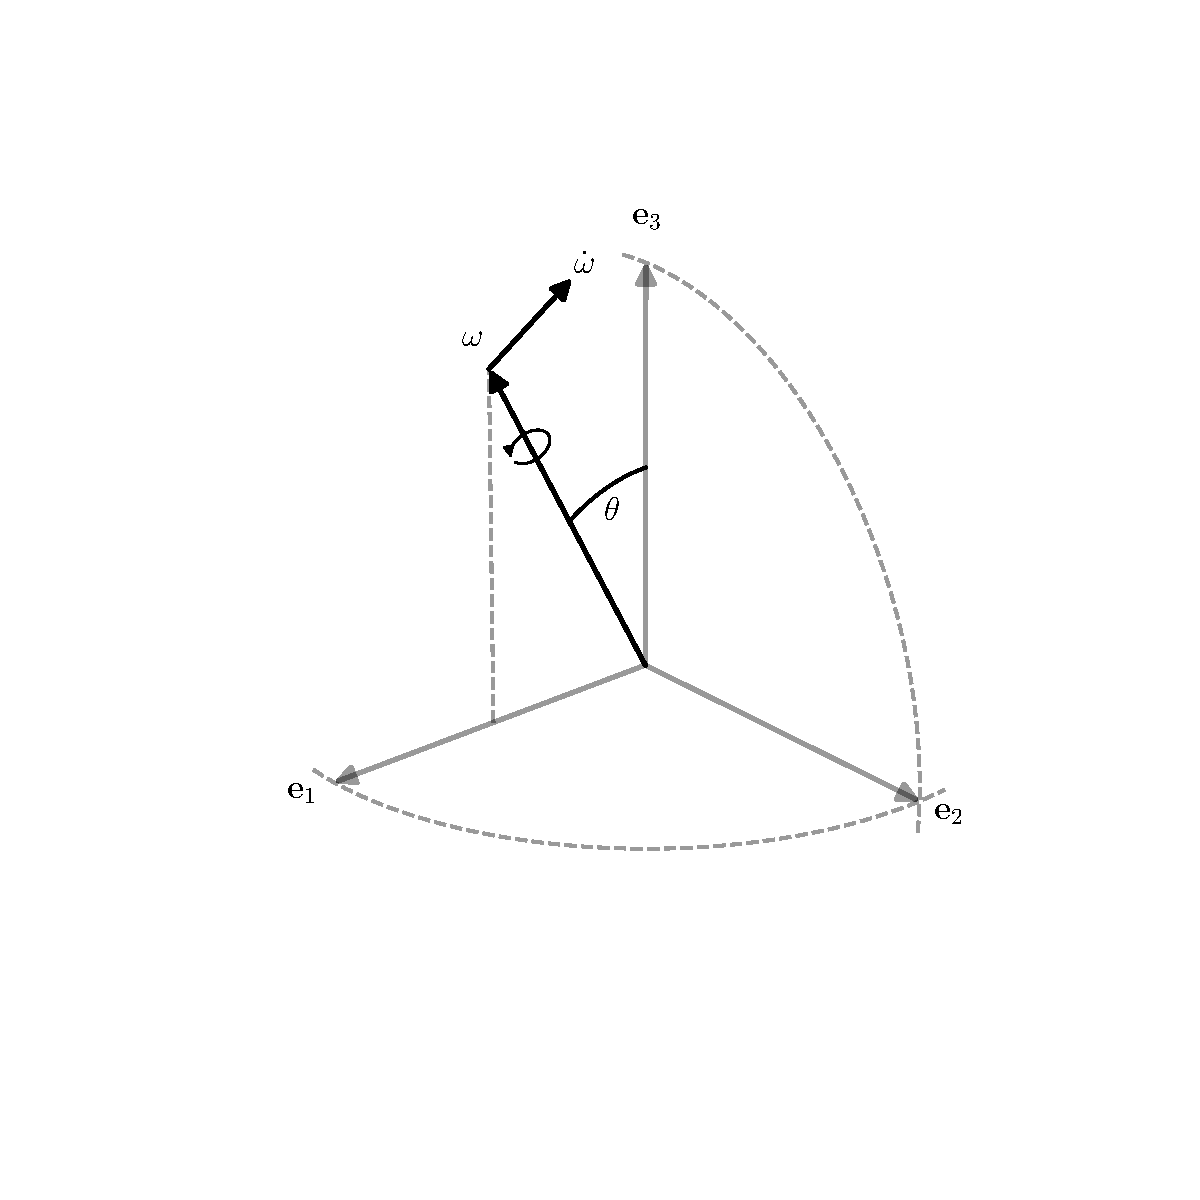
\includegraphics[width=0.9\textwidth]{figures/reference_frames.pdf}
\caption{Relevant vectors and angles for the TPW analysis. The axes $\mathbf{e}_1$, $\mathbf{e}_2$, and $\mathbf{e}_3$ represent the principal axes of the convective moment of inertia $\mathbf{E}$, with associated eigenvalues $\lambda_1$, $\lambda_2$, and $\lambda_3$, respectively.  The angle $\theta$ represents the mismatch between the rotation axis $\mitbf{\omega}$ and the $\mathbf{e}_3$-axis. For illustration, the longitude $\phi$ of the rotation axis is taken to be zero so $\mitbf{\omega}$ lies in the $\mathbf{e_1}$-$\mathbf{e_3}$ plane. In general $\phi$ is not zero. True polar wander moves the rotation axis towards the $\mathbf{e}_3$-axis. Observations of $\dot{\mitbf{\omega}}$ are made in the geographic frame, which drifts relative to the E-frame.  }
\label{fig:reference_frames}
\end{figure*}

The second special case occurs when the rotation vector $\mitbf{\omega}$ lies in $\mathbf{e}_1$-$\mathbf{e}_3$ plane ($\phi = 0$).
Equation~\eqref{eq:polar_wander_rate} reduces to
\begin{equation}
\vert \dot{W} \vert = 
\frac{1}{2(C-A) \tau_R}\sin{2\theta} ( \lambda_3 - \lambda_1)\, .
\label{eq:simple_milankovitch}
\end{equation}
An equivalent expression was given by \citet{tsai2007theoretical}. We adopt Equation (17) as the basis for our dimensional analysis. Note that
the maximum  rate is achieved when $\theta=45^\circ$ (see, e.g. \citet{fung1965foundations}).

From Equation~\eqref{eq:simple_milankovitch} it is clear that the important quantities for estimating the rate of true polar wander ($\dot{W}$)
are $\theta$ and $\lambda_3 - \lambda_1$. Both of these quantities depend on the structure and dynamics of mantle convection.  The size of
convective anomalies directly determines $\mathbf{E}$, and hence $\lambda_3-\lambda_1$. We also expect convection to alter the orientation of the principal axes of $\mathbf{E}$, which drives a change in $\theta$. Relaxation of the rotation axis back toward the principal axis of $\mathbf{E}$ acts to reduce $\theta$. In the next section we focus on the role of mantle convection in setting $\lambda_3-\lambda_1$ and in driving changes in $\theta$.



\section{Internal dynamics}
\label{sec:internal}

Mantle convection and rotational dynamics of planetary bodies are usually considered separately, yet the processes are based on a common set of governing equations. 
As such, some extra care must be taken to ensure that the equations we consider are self-consistent. 
Furthermore, since our goal is to establish a scaling for TPW rate, we must identify a minimal set of nondimensional numbers that fully characterize the problem.
For simplicity we consider an isoviscous planet in a rotating reference frame with no internal heating in the incompressible Boussinesq approximation.  The equations for mass, momentum, and energy then read

\begin{equation}
\nabla \cdot \mathbf{u} = 0
\label{eq:conserve_mass}
\end{equation}

\begin{equation}
\begin{aligned}
- \nabla P + \eta \nabla^2 \mathbf{u} =  \rho \mathbf{g} -  \rho \mitbf{\Omega} \times \mitbf{\Omega} \times \mathbf{r}
\label{eq:navier_stokes}
\end{aligned}
\end{equation}

\begin{equation}
\frac{\partial T}{\partial t} + \mathbf{u} \cdot \nabla T = \kappa \nabla^2 T
\label{eq:energy}
\end{equation}
where $\mathbf{u}$ is the velocity, $P$ is the pressure, and $T$ is the temperature.
The vector $\mathbf{g}$ is the gravitational acceleration, 
which defined in terms of a gravitational potential $V$ by $\mathbf{g} = -\nabla V$. 
The gravitational potential obeys 
\begin{equation}
\nabla^2 V = 4 \pi G \rho.
\end{equation}
where $G$ is the gravitational constant. 
For the purposes of scaling, we assume that the magnitude of the gravitational acceleration, $g_0$, is approximately constant (as is the case for Earth's mantle).
In addition we use the simple equation of state
\begin{equation}
\rho = \rho_0 \left( 1 - \alpha (T-T_0) \right).
\label{eq:eos}
\end{equation}
to define the density.
The remaining parameters are defined in Table~\ref{tab:parameters}.
Note that we retain the centrifugal term in the momentum equation, which is normally either neglected or absorbed into a modified pressure
(in the latter case the boundary conditions on $P$ must be modified).
The centrifugal term
is generally small compared to gravitational forces (at least for Earth-like parameters). Consequently, it does  not have a strong influence on the style of convection.
However, this term is critical for determining the size of the rotational bulge. It is also essential for establishing a connection between the linear and angular momentum equations.

Four dimensionless parameters are required to characterize the dynamics of true polar wander  (cf. \citet{barenblatt1996scaling}). A fifth parameter, defined  by the ratio of the length of day to a diffusion timescale, does not appear in the governing equations.
Convenient choices for these numbers are listed in Table~\ref{tab:nondim}, along with approximate Earth-like values for them. This particular choice relies on $R$ for the length scale, $R^2/\kappa$ for the time scale and $\Delta T$ for the temperature scale.

Two of these four dimensionless parameters have a prominent role in our scaling analysis. 
The first is the Rayleigh number, which characterizes the  vigor of convection. 
The second is the ratio of centrifugal to gravitational forces.
This nondimensional number does not have a uniformly agreed-upon name: 
it has been called a Froude number in analogy with other applications of inertial-to-gravitational effects \citep{mckenzie1968influence}, 
and in the geodesy community has commonly been termed $m$ \citep[e.g.][]{nakiboglu1982hydrostatic, chambat2010flattening}, which we adopt here.
Since we have begun with equations that do not have inertia or compressibility, we have implicitly thrown out the dependence on the nondimensional numbers that characterize those effects (e.g., the Prandtl and dissipation numbers).
It would be straightforward to include them, but they do not affect the overall treatment of this scaling.

The dynamics can be characterized in terms of deviations from a reference hydrostatic state. We define a
 dynamic pressure by $P^* = P - P_0$ and introduce density perturbations $\delta \rho = \rho- \rho_0 = - \rho_0 \alpha (T-T_0)$.
In addition, we expect deviations in the figure of the planet from its hydrostatic shape, 
which we denote by $V = V_H + \Delta V$, where $V_H$ is the hydrostatic figure and $\Delta V$ is the deviation. 
Our rationale for this decomposition is simply that the hydrostatic pressure is defined in the hydrostatic configuration $V_H$ rather than $V$. 
Introducing $\Delta V$ requires another nondimensional number to characterize it, 
and we find that the quantity $\Gamma \equiv \alpha \Delta T$ is convenient. (The motivation for this choice is explained below.)
Finally, we define $\mitbf{\Omega} = \Omega_0 \mitbf{\omega}$, where $\mitbf{\omega}$ is a unit vector in the direction of $\mitbf{\Omega}$.

By definition the hydrostatic reference state is a solution to Equation~\eqref{eq:navier_stokes} where there is no flow:
\begin{equation}
\begin{aligned}
- \nabla P_0 =  \rho_0 \mathbf{g} -  \rho_0 \mitbf{\Omega} \times \mitbf{\Omega} \times \mathbf{r}.
\label{eq:hydrostatic}
\end{aligned}
\end{equation}
Removing this reference state from the full momentum equation defines an equation for the perturbations. 
When the perturbed momentum equation is written in nondimensional form using the parameters in Table~\ref{tab:nondim} we obtain:
\begin{equation}
\begin{aligned}
 - \nabla P^* + \; \nabla^2 \mathbf{u} - \mathrm{Ra} \; T \; \mathbf{g} + \mathrm{Ra} \; m \; T \;{\mitbf{\omega} \times \mitbf{\omega} \times \mathbf{r}} = 0.
\end{aligned}
\end{equation}
Only two dimensionless parameters appear in Equation (24); the buoyancy force is specified by $Ra$ and the centrifugal force depends on the product $Ra\; m$.
No additional parameters appear in the energy (temperature) equation because $\Delta T$ is used to scale temperature and time is scaled by the thermal diffusion time $\tau_T = R^2/\kappa$.
The aspect ratio $A$ arises in the problem through definition of the boundary conditions, whereas the dependence on the dimensionless density deficit $\Gamma$ has not yet emerged. This dependence is
revealed by drawing a connection between the linear and angular momentum equations. 

We start with the dimensional form of 
Equation~\eqref{eq:navier_stokes}.  Crossing it with $\mathbf{r}$ and integrating over the volume of the mantle gives:
\begin{equation}
\begin{aligned}
-\int_V \mathbf{r} \times \nabla P \,dV + \int_V \eta \mathbf{r} \times \nabla^2 \mathbf{u} \,dV - \int_V \rho \mathbf{r} \times \mathbf{g} \,dV 
   + \int_V \rho \mathbf{r} \times \mitbf{\Omega} \times \mitbf{\Omega} \times \mathbf{r}  \,dV &= 0. \\
\end{aligned}
\end{equation}
The first three terms represent pressure, viscous torques, and gravitational torques on the mantle.  
Convection in the outer core, atmospheres, and oceans is not strong enough to provide significant pressure and viscous torques over geologic timescales, and a self-gravitating body cannot self-torque \citep{braginsky1995equations}.
Therefore we can neglect those terms, and we are left with
\begin{equation}
\begin{aligned}
\int_V \rho \mathbf{r} \times \mitbf{\Omega} \times \mitbf{\Omega} \times \mathbf{r} \,dV &= 0 \\
\label{eq:quasistatic_angular_momentum}
\end{aligned}
\end{equation}
which may be rewritten via the Jacobi identity to find
\begin{equation}
\begin{aligned}
 \mitbf{\Omega} \times \int_V \rho \mathbf{r} \times (\mitbf{\Omega}\times \mathbf{r}) \,dV &= 0. \\
\end{aligned}
\end{equation}
This equation can be directly identified with Equation~\eqref{eq:quasistatic_liouville}; it 
 is a statement that a quasistatic body will rotate around the principal axis of its total moment of inertia.

We now seek to quantify the perturbation to Equation~\eqref{eq:quasistatic_angular_momentum} due to dynamics.
Hydrostatic balance (Equation~\eqref{eq:hydrostatic}) ensures that the integral over the reference shape $V_H$ vanishes when $\rho = \rho_0$.
Nonzero contributions arise from perturbations in the density field or from perturbations in the shape.
To make this dependence explicit, we split the shape into the reference volume $V_H$ and perturbations from it $\Delta V$,
and use Equation~\eqref{eq:eos} to define density perturbations.
Substituting this decomposition into Equation~\eqref{eq:quasistatic_angular_momentum} brings the integral into the form
\begin{equation}
\begin{aligned}
&\int_{V_H} \rho_0 \mathbf{r} \times \mitbf{\Omega} \times \mitbf{\Omega} \times \mathbf{r} \,dV + 
\int_{V_H} \rho_0 \alpha (T-T_0) \mathbf{r} \times \mitbf{\Omega} \times \mitbf{\Omega} \times \mathbf{r} \,dV +  \\
&\int_{\Delta V} \rho_0 \mathbf{r} \times \mitbf{\Omega} \times \mitbf{\Omega} \times \mathbf{r} \,dV + 
\int_{\Delta V} \rho_0 \alpha (T-T_0) \mathbf{r} \times \mitbf{\Omega} \times \mitbf{\Omega} \times \mathbf{r} \,dV = 0.  \\
\end{aligned}
\end{equation}
As previously noted, the first term of this equation is zero due to the hydrostatic equation.  
The fourth term is negligible due to being second order in the smallness parameters $\Delta V/V_H$ and $\Gamma\equiv \alpha \Delta T$.
Removing these, we find
\begin{equation}
\begin{aligned}
\int_{\Delta V} \rho_0 \mathbf{r} \times \mitbf{\Omega} \times \mitbf{\Omega} \times \mathbf{r} \,dV = 
-\int_{V_H} \rho_0 \alpha (T-T_0) \mathbf{r} \times \mitbf{\Omega} \times \mitbf{\Omega} \times \mathbf{r} \,dV.
\end{aligned}
\end{equation}
This equation may be identified with Equation~\eqref{eq:disequilibrium}, 
where disequilibrium in the rotational deformation (left side) is balanced by the mismatch of the convective moment of inertia with the spin axis (right side). Equation (29) also reveals
the need for  the dimensionless parameter $\Gamma = \alpha \Delta T$. The perturbation  $\alpha(T-T_0)$ on the right-hand side must be related to the perturbation $\Delta V$ on the left-hand side because all other terms in Equation (29) are the same. A change in the scale of $\Delta V$ implies a change in the scale of $\alpha(T-T_0)$, and vice versa. 

We now proceed to characterize the rate of TPW in terms of the dimensionless number identified in Table~\ref{tab:nondim}. This approach ensures that we reduce the problem to the minimum set of parameters.



\begin{table}
\centering
\caption{Parameters for rotating mantle convection}
\label{tab:parameters}
\begin{tabular}{@{}lcc}
Symbol & Definition\\
\hline
$R_i$ & inner radius \\
$R$ & outer radius \\
$G$ & gravitational constant \\
$V$ & gravitational potential \\
$M$ & mass of the planet \\
$\Omega_0$ & reference rotation rate \\
$\eta$ & viscosity \\
$\kappa$ & thermal diffusivity \\
$\alpha$ &  thermal expansivity \\ 
$g_0$ & reference gravity \\
$I_0$ & reference moment of inertia \\
$T_0$ & reference temperature \\
$\rho_0$ & reference density \\ 
$\Delta T$ & temperature drop across mantle
\end{tabular}
\end{table}

\begin{table}
\centering
\caption{Nondimensional numbers with approximate Earth-like values}
\label{tab:nondim}
\begin{tabular}{@{}lcccc}
Symbol &  Name & Definition & Approximate value \\
\hline
Ra & Rayleigh &  $\rho_0 g_0 \alpha \Delta T R^3/\eta \kappa$ & $10^7$\\
$m$ & Froude & $\Omega_0^2 R/g_0 = \Omega_0^2 R^3/GM$ & $10^{-3}$ \\
A & aspect ratio & $R_i/R$ & $0.54$ \\
$\Gamma$ & density deficit &$ \alpha \Delta T$ & $10^{-2}$ \\
\end{tabular}
\end{table}
 
\section{Scaling}
\label{sec:scaling}

Equation (17) defines the rate of TPW in terms of four physical parameters: $(C-A)$, $\tau_R$, $(\lambda_3-\lambda_1)$ and $\theta$. This equation can be expressed in nondimensional form using the dimensionless numbers from Table 2. We begin by expressing $\dot{W}$ in terms of a nondimensional time $t^{\prime} = t /\tau_T$, where $\tau_T = R^2/\kappa$ is the thermal diffusion time. Similarly, the time constant $\tau_R$ can be expressed in terms of $\tau_T$ and other dimensionless numbers. In detail $\tau_R$ represents a weighted average of different relaxation modes, but it is sufficient for our purposes to let
\begin{equation}
\tau_R \sim \frac{ \eta }{ \rho_0 g_0 R} = \tau_T \, \frac{\Gamma}{\mathrm{Ra} }.
\end{equation}
Combining these results gives the dimensionless rate of TPW
\begin{equation}
\frac{dW}{dt'} \sim \frac{Ra}{\Gamma} \frac{(\lambda_3 - \lambda_1)}{(C-A)} \sin 2\theta\, .
\end{equation}
A more convenient form is obtained by noting that difference in the polar and equatorial moments $(C-A)$ is proportional to the ratio of rotational to gravitational forces
\citep{munk1960rotation}:
\begin{equation}
(C-A) \sim I_0 m.
\end{equation}
We can also define a nondimensional eigenvalue differencing using $\Lambda_{ij} = (\lambda_i-\lambda_j)/I_0$. Introducing these results into Equation (31) gives
\begin{equation}
\frac{d W}{dt'} \sim \frac{Ra\, \Lambda_{31}}{\Gamma\, m} \sin 2\theta
\end{equation}
which defines the rate of TPW in terms of dimensionless parameters $Ra$, $m$ and $\Gamma$. At this point we do not have estimates for $\Lambda_{ij}$ or $\theta$.  However, we do know that they must be functions of the dimensionless numbers in Table 2 and our dimensionless time $t^{\prime}$.


For the case of slowly rotating bodies ($m \ll 1$), we do not expect rotation have a large influence on the style of convection, so it would be reasonable to  
 look for scalings of the form $\Lambda_{ij}(\mathrm{Ra}, \Gamma, t^{\prime})$ and $\theta(\mathrm{Ra}, \Gamma, t^{\prime})$. We avoid the complications of dealing with the time dependence by considering time averages for $\Lambda_{ij}$ and characterizing an upper bound on $\theta$.


\subsection{An estimate for $\Lambda_{ij}$}
\label{sec:lambda}


Fluctuations in the nonhydrostatic moment of inertia are caused by a redistribution of density anomalies 
 in the mantle. The direct contribution from 
internal temperature variations is given by
\begin{equation}
C_{ij} = \int_{V_H} \rho_0 \alpha (T-T_0) \left( r_q r_q \delta_{ij} - r_i r_j \right) \,dV
\label{eq:temperature_fluctuations}
\end{equation}
An additional contribution arises from the deflection of the surface and internal interfaces. The surface response is a function of the viscosity structure of the planet and the wavelength and depth of the internal load. It is customary to represent the surface response using the fluid-limit geoid kernals,  where the factor
 $1+k^L_f$ is close to 1. 
(Strictly speaking, dynamic compensation usually makes $1 + k_f^L$ less than one, \citep[e.g.][]{richards1984geoid}). 
For the purposes of scaling, we can omit this multiplicative factor and estimate $E_{ij}$ from the direct contribution $C_{ij}$.

For thermal convection, the convective part of the moment of inertia is related to the degree-two part of the temperature field (see Appendix A).
To extract this component of the temperature field we can expand $T-T_0$ in a sum  of orthonormal basis functions $R_n Y_{lm}$, 
where $Y_{lm}$ are spherical harmonics and $R_n$ are some set of orthogonal radial polynomials. The coefficients
$T_{nlm}$ of the series expansion are normalized by $\Delta T$, so we represent the temperature anomaly in the form
\begin{equation} 
T( r , \theta, \phi, t ) - T_0 = \Delta T {\displaystyle \sum_{n=0}^\infty \sum_{l=0}^\infty \sum_{m=-l}^{l} } T_{lmn}(t) R_n(r) Y_{lm} (\theta , \phi).
\label{eq:T_series}
\end{equation}
Orthogonality of the basis functions means that the integral for $C_{ij}$ picks out degree-two 
spherical harmonics in the lateral dimensions, and only the lowest few radial functions $R_n(r)$.
Consequently, only a few terms in the expansion matter for TPW.
We seek to estimate the power in those few modes, which we denote by $T_{\text{degree-two}}$ (see Appendix A for more detail). Once the contribution to $T_{\text{degree-two}}$ is established, the integral for $C_{ij}$ can be approximated by
\begin{equation}
C_{ij} \sim I_0 (\alpha \Delta T) T_{\text{degree-two}} \, .
\end{equation}
The nondimensional difference in the principal moments becomes
\begin{equation}
\Lambda_{31} \sim \Gamma T_{\text{degree-two}}.
\end{equation}

Normalizing the 
 temperature field by $\Delta T$ means the summation over all basis functions in Equation (35) cannot exceed 1. This is a strong constraint, but it gives very little information about the distribution of power across the $T_{lmn}$.  
We can, however, think about the power spectrum in two different regimes: that of steady/quasisteady flow, (relatively low $\mathrm{Ra}$) 
and that of chaotic flow (relatively high $\mathrm{Ra}$). At low Rayleigh number we expect the spectrum of the temperature field to be dominated by only a few low-degree modes which are largely influenced by the aspect ratio. At high Rayleigh number become chaotic and there is a broadening of the spatial and temporal spectra  \citep{mclaughlin1982transition}.  

\begin{figure*}
\centering
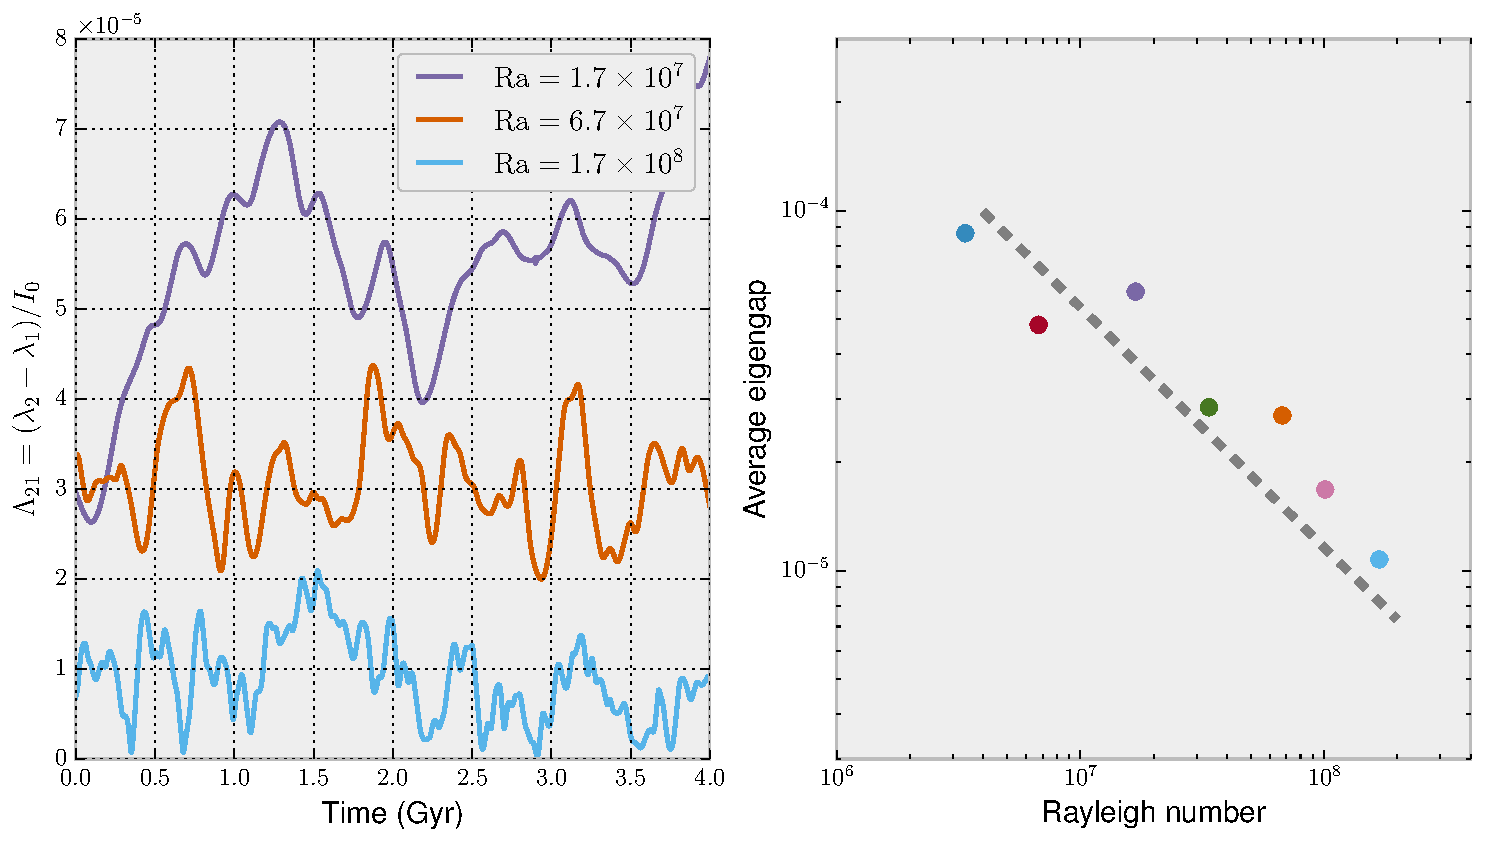
\includegraphics[width=0.9\textwidth]{figures/eigengap.pdf}
\caption{ Left: Time series of the normalized difference between moments $\Lambda_{21} = (\lambda_2 - \lambda_1)/I_0$ for convection in a 2D annulus at several different Rayleigh numbers.  As the Rayleigh number increases, the average value of the relative moment decreases due to less low-degree coherence in the temperature structure.  Right:  average value of $\Lambda_{21}$ for the different Rayleigh numbers.  Also shown is a line with slope $\mathrm{Ra}^{-2/3}$, which is predicted from the scaling analysis (the exponent is $-2/3$ instead of $-1$ due to the reduced dimensionality of the simulations).}
\label{fig:eigengap}
\end{figure*}

The lengthscale of temperature anomalies in the mantle is limited by the effects of thermal diffusion. 
Structure at very short lengthscales is erased by thermal diffusion, so there will be little power in modes
with lengthscales shorter than that allowed by diffusion. 
Therefore the infinite sum in Equation~\eqref{eq:T_series} can be truncated at some maximum wavenumber, set by the smallest lengthscale $d$:
\begin{equation}
n_{\text{max}}, l_{\text{max}}, m_{\text{max}} \sim \frac{R}{d}.
\label{eq:max_wavenumber}
\end{equation}
Strictly speaking, convective mixing can produce smaller scales, but the power in these scales
is greatly reduced by diffusion.
Thus total number of modes that are accessible to the system are 

\begin{equation}
N_{\text{modes}} = n_{\text{max}} \times l_{\text{max}} \times m_{\text{max}} \sim \left( \frac{R}{d} \right)^{3}.
\end{equation}
The value of each $T_{lmn}(t)$ will in general be some complex function of time, but for a given style of convection we expect the time average to define a representative power spectrum.
For chaotic flow the power should be spread out amongst the modes accessible to it.
We may make the hypothesis that each of the modes are roughly as likely as any of the others, which implies

\begin{equation}
T_{\text{degree-two}}(t) \sim \frac{1}{N_{\text{modes}}} \sim \left( \frac{d}{R}\right)^3.
\label{eq:degree_two_of_lengthscale}
\end{equation}

Any of a number of scaling laws can provide an estimate for the characteristic length scale of a convecting system. The specifics are likely to depend on rheology, geometry, and density structure.
The simplest model is based on boundary layer theory \citep{turcotte1967finite}, which finds $d/R \sim \mathrm{Ra}^{-1/3}$.
This scaling is roughly a measure of the diffusive lengthscale for the timescale of a convective overturn, consistent
with the cutoff in Equation~\eqref{eq:max_wavenumber}.
It thus furnishes us with an estimate of the power in 
the degree-two part of the field as a function of Rayleigh number:

\begin{equation}
T_{\text{degree-two}}(t) \sim \mathrm{Ra}^{-1}.
\label{eq:degree_two_of_ra}
\end{equation}

We test this prediction using a series of numerical simulations of mantle convection at different Rayleigh numbers. 
All calculations are based on the mantle convection software \texttt{ASPECT} \citep{kronbichler2012high}, which is built on the finite element library \texttt{deal.II} \citep{dealII82}. This package
 allows for flexible implementation of different rheologies, geometries, and postprocessors.
In order to test a wide range of Rayleigh numbers, we ran the simulations in a 2D annulus. At each time step we evaluate moment of inertia tensor in the frame of the convection calculation and evolve an initial rotation vector in time using  Equation~\eqref{eq:liouville_ode}. Recall that Equation (13) describes the evolution of the rotation vector in a geographic frame. Here we adopt the coordinate frame of the convection calculations as the geographic frame, so off-diagonal elements of $\mathbf{E}$ will generally be non-zero. We also calculate the eigenvalues of $\mathbf{E}$ at each time step to evaluate $\Lambda_{21} = (\lambda_2 - \lambda_1)/I_0$.

For the 2D simulations there is a reduced dimensionality when calculating the number of modes,
so $N_\text{modes} \sim \left(R/d \right)^2$.  This leads us to a scaling of $T_{\text{degree-two}} \sim \mathrm{Ra}^{-2/3}$ and $\Lambda_{21} \sim \Gamma Ra^{-2/3}$, according to Equation (37).  A fit to the average value of $\Lambda_{21}$ as a function of $Ra$ is shown as a dashed line in Figure~\ref{fig:eigengap}.
This result has a simple interpretation.
As the Rayleigh number of the system increases, the smallest lengthscale of convective features gets smaller.
The total power in the temperature field is spread across a larger spectrum, leaving less total power for the degree-two part to drive TPW.


Returning to the three-dimensional problem we expect $\Lambda_{ij}$ to scale as
\begin{equation}
\Lambda_{ij} \sim \frac{\Gamma}{\mathrm{Ra} }.
\label{eq:lambda_estimate}
\end{equation}
Using this estimate in Equation (33) gives
\begin{equation}
\frac{d W}{dt^\prime} = \frac{1}{m} \sin 2 \theta
\end{equation}
Remarkably, $Ra$ and $\Gamma$ have completely dropped from the expression for the rate of TPW.  The time constant $\tau_R$ goes down at high Rayleigh numbers. At the same time, the  coherence in the temperature structure goes down, reducing the amount of power in the degree-two part of the field responsible for driving TPW.
\citet{tsai2007theoretical} arrive at a similar result by a different path.
Their estimate for the ratio of the convective timescale to the timescale for TPW depends only on $m$ (see their Equation~(4)).
That the two results are similar is surprising, as their estimate of $T_\text{degree-two}$ varies linearly with $d/R$,
rather than with $(d/R)^3$ (Equation~\eqref{eq:degree_two_of_lengthscale}).

The cancellation of explicit $\mathrm{Ra}$ dependence is something of a coincidence due to the simple estimate of the smallest lengthscales of the problem.
Scalings for lengthscales of convection in fluids with temperature dependent viscosity \citep[e.g.][]{solomatov1995scaling} or pseudoplastic rheology \citep[e.g.][]{korenaga2010scaling} have different functional dependencies on $\mathrm{Ra}$ or additional nondimensional parameters.
However, a common feature in most scalings is that typical lengthscales are still some power-law of Rayleigh number $d \propto \mathrm{Ra}^{-\beta}$.
With this form, our scaling for TPW rate has the following dependence on $\mathrm{Ra}$:
\begin{equation}
\frac{d W}{dt^\prime} \sim \frac{\mathrm{Ra}^{1-3\beta}}{m} \sin{2 \theta}.
\label{eq:simplest_milankovitch_defer_scaling}
\end{equation}
In general, $\beta$ is some small number between one-fourth and one-third, so we expect that more complicated estimates for 
$d(\mathrm{Ra})$ will still result in a weak dependence 
on the Rayleigh number.

\subsection{An estimate for the angular mismatch angle ($\theta$)}
\label{sec:theta}

Much of the debate about the magnitude of TPW on Earth comes down to the question of how big $\theta$ can be.
\citet{kirschvink1997evidence} hypothesized about an inertial interchange event, where $\theta$ alters by approximately 90$^\circ$,
and can lead to large ($\sim90^\circ$) TPW over time (a process which they termed ``inertial interchange'' TPW, or IITPW).
Conversely, many geodynamic simulations of recent TPW assume that $\theta$ is small \citep{steinberger1997changes}.
In this section we seek to characterize the maximum value for $\theta$ in terms of the dimensionless parameters.

Two processes control the evolution of $\theta$. It grows through perturbations in the convective moment and  decays by relaxation of the rotation axis towards the principal axis of $\mathbf{E}$. Large values of $\theta$ are achieved when
convective perturbations deflect the principal axis away from the rotation axis faster than relaxation can reduce $\theta$. Here we focus on the nature of
perturbations that drive large increases in $\theta$ with the understanding that a complete description of $\theta(t)$ as a function of time must include both the growth and decay of the misalignment. 

An instantaneous change in the convective moment of inertia shifts the orientation of the principal axis, causing a change in the misalignment angle. A random change could make the angle larger or smaller, so there is no guarantee that a given perturbation will cause $\theta$ to grow. On the other hand,  we know that $\theta$ only grows through perturbation in the convective moment. Of course no change in the moment of inertia happens instantaneously. Instead,  changes in $\mathbf{E}$ accumulate over  finite durations and these gradual changes must compete with the relaxation process to define the evolution of $\theta$. Still, the concept of an instantaneous perturbation is useful because the conditions that facilitate large changes in $\theta$ also promote rapid growth rates. 

Given a random perturbation to $\mathbf{E}$, we would like to give a bound on the size of changes in the orientation of the principal axes. Let $\delta$ be the size of the perturbation to the convective moment of inertia tensor after some time interval $\Delta t$, and let $\lambda_3 \ge \lambda_2 \ge \lambda_1$ be the eigenvalues of that tensor.  The corresponding rotation of the principal axes is defined by the angle $\xi$. A bound on $\xi$ is given by \citep{davis1970rotation}
\begin{equation}
\vert \sin(2 \xi) \vert \le \frac{ 2 \vert \delta \vert}{ \displaystyle \min_{i \neq j} \vert \lambda_i - \lambda_j \vert }.
\label{eq:kahan}
\end{equation} 
Small changes in orientation (i.e. small $\xi$) occur when the difference in eigenvalues is large. Conversely, large changes in orientation are possible when differences between the eigenvalues are small. 
This dependence is illustrated schematically in Figure~\ref{fig:perturb}.  Unstable conditions prevail when the maximum and intermediate moments of inertia are nearly equal, leading to large TPW events \citep{evans1998true}. On the other hand, \citet{tsai2007theoretical} point out that large TPW events take a long time because the rate of TPW is small when $\Lambda_{31}$ is small or when $\theta = 0$ or $\pi/2$ (see Equation (33)). If the maximum and intermediate axes are interchanged when the misalignment angle is small $\theta \approx 0$, then the new definition of the maximum axis after the interchange ensures that $\theta \approx \pi/2$. In this case the rate of TPW may be small before and after the interchange.

\begin{figure*}
\centering
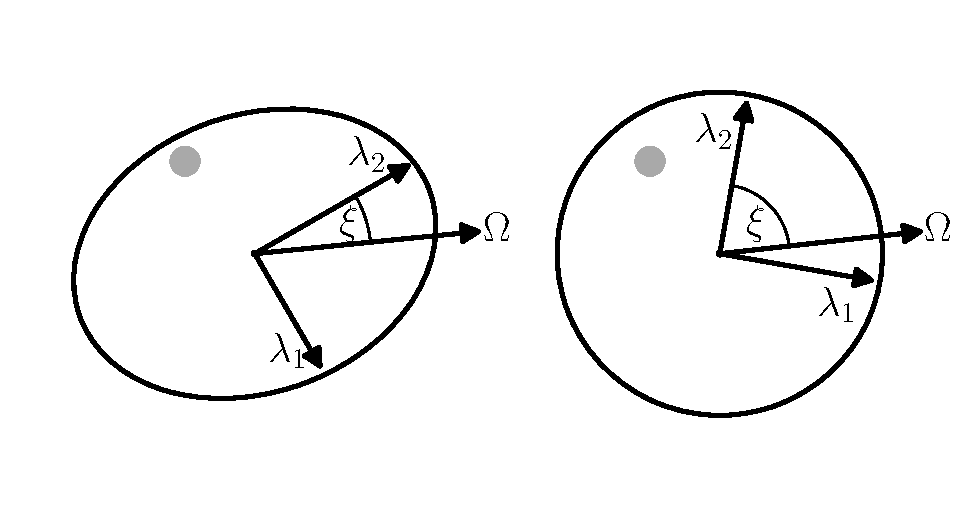
\includegraphics[width=0.9\textwidth]{figures/perturb.pdf}
\caption{Graphical demonstration of the $\sin{2 \xi}$ theorem of \citet{davis1970rotation}.  Two spheroidal bodies with eigenvalues $\lambda_2 > \lambda_1$ start out with the rotation axis $\Omega$ aligned with the $\lambda_2$ axis. However, on the left the eigengap $\lVert \lambda_2 - \lambda_1 \rVert$ is large, while on the right it is small.  A negative mass perturbation is instantaneously added to both bodies, which effects a small rotation of the principal axes on the left, but a large one on the right.}
\label{fig:perturb}
\end{figure*}

The angle $\xi$ would correspond to a change in $\theta$ if relaxation was not allowed to operate. While this approximation is not realistic, it does suggest that larger perturbations in $\theta$ are possible when  $(\lambda_i-\lambda_j)$ small. Scaling results and numerical simulations from the previous section show that the difference in eigenvalues scales with $\sim \mathrm{Ra}^{-1}$.
Therefore, the characteristic gap between the eigenvalues of the convective moment becomes smaller as the Rayleigh number increases.
Additionally, the timescale of fluctuations in these values goes down because the density anomalies are moving faster.
Overall, this makes the principal axes of high Rayleigh number systems much less stable, consistent with the result of \citet{richards1999polar}, based on mantle convection calculations.

In the limit that the eigengap becomes zero, a small perturbation $\delta$ can produce an arbitrary rotation of the principal axes. In effect, the location of the principal axes are set by the location of a small density anomaly. This has a close correspondence with hypothesized IITPW \citep{kirschvink1997evidence}. As noted above, the interchange of the maximum and intermediate axex can produce a large change in $\theta$ because the misalignment angle is suddenly measured from a new axis. The resulting TPW event can produce a large change in the orientation of the rotation axis (potentially $90^{\circ}$ if there are not further perturbations to the $\mathbf{E}$ tensor).  However, the eigengap does not need to be zero for there to be large polar wander events. In addition, wander does not need to be $90^\circ$ after an interchange of maximum and intermediate axes due to the subsequent evolution of density anomalies during the event.  We clarify these points using numerical simulations of convection in a 2D spherical annulus.

Figure~\ref{fig:misfit} shows a representative time series from the convection calculations. As before, we compute the convective moment of inertia in the geographic frame and evaluate the eigenvalues of $\mathbf{E}$ to determine the eigengap. We also evolve the orientation of the rotation axis by integrating  Equation~\eqref{eq:liouville_ode} in time.
Since it is a 2D model, the spin axis is described by a single angle. The misalignment angle $\theta$ also lies in the plane of the 2D model.
When the eigengap gets small,  the corresponding misalignment angle increases.
Even though at that moment the driving force may be small,
it can recover quickly due to convection, and the rate of polar wander becomes much faster.
This behavior is consistent with the predictions from Equation (33). We draw special attention to two events in the time series. At $\sim$0.3 Gyr the eigengap dips and the misalignment angle increases to $\theta \sim 20^{\circ}$. There is a large change in the orientation of the spin axis, even though
there is technically no interchange of the maximum and intermediate axes. A conventional IITPW event occurs at $\sim 1$ Gyr;  the eigengap goes to zero, interchanging the maximum and intermediate axes. The misfit angle goes to approximately $90^\circ$. During this time the orientation of the spin axis changes by roughly 90$^{\circ}$. 

Large TPW events are associated with inertial interchanges, but a broader class of events are evident
when the principal moments are close to each other. We argue that large TPW events do not (necessarily) imply an inertial interchange. Conversely, we do not expect all large TPW events to be associated with a 90$^{\circ}$ change in the spin axis. Our scaling results suggest that large TPW events are more likely to occur in the early Earth when the planet is convecting more vigorously and the characteristic gap between principal moments is small.


\citet{tsai2007theoretical} suggested that large TPW events do not always accompany an interchange of the principal moments because the rate of TPW is low. A large 90$^{\circ}$ change in the orientation of the rotation axis can only occur over a long time.  While
this is true for idealized cases, the numerical convection calculation reveals a more complex behavior. 
First, the principal moments can interchange, or almost interchange, quite rapidly. In these cases  the perturbations in the convective moments can become large soon after an interchange.
Second, the location of the principal axes do not stay put during a IITPW event. A persistent drift of the principal axes can can lead to extended polar wandering, yielding angular changes greater than 90$^\circ$.

\begin{figure*}
\centering
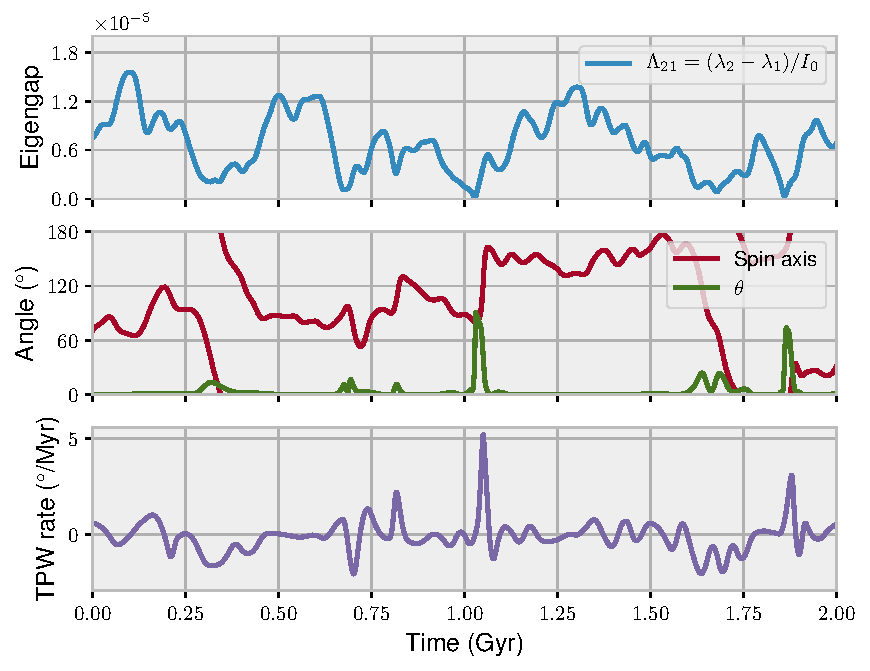
\includegraphics[width=0.9\textwidth]{figures/misfit.pdf}
  \caption{Top: Time series of principal moments for 2D annular convection at $\mathrm{Ra}\sim10^8$.  Center: Time series of spin axis and mismatch angle $\theta$.  Bottom: Time series of TPW rate. When the two moments are close to each other (small eigengap), the mismatch angle becomes large, and the rate of polar wander is significantly larger. At $\sim$1 Gyr the gap goes to zero and there is a nearly $90^\circ$ TPW event, with $\sim80^\circ$ degrees of polar wander in $\sim$30 Myr. However, there are several other large TPW events which happen when the eigengap is small. These results are fairly characteristic of high $\mathrm{Ra}$ convection.}
\label{fig:misfit}
\end{figure*}


\section{Discussion}
\label{sec:discussion}

The preceding results clarify the complex relationships that determine the rates of TPW for a convecting planet.
As mantle convection redistributes mass in the planet's interior, the spin axis moves around to stay aligned with the principal axes of the convective moment of inertia. 
There is a constant competition between growth of the mismatch angle $\theta$ through convective perturbations
 and its relaxation through TPW.
\citet{goldreich1969some} envisioned an analogy of beetles crawling on the surface of the globe, with
the spin axis trying to keep up with the instantaneous figure axis set by the beetles.
Our analysis begins to answer the questions ``how big are the beetles?'' and ``how fast are they crawling?''. We find that the most important parameters are $m$, which acts as the brakes on the system, and the mismatch angle $\theta$. Surprisingly, the direct dependence of $\dot{W}$ on $Ra$ is weak (see Equation (44)), but the indirect influence of $Ra$ on the misalignment angle $\theta$ is quite strong.

Indeed, we can identify two endmember behaviors of Equation~\eqref{eq:simplest_milankovitch_defer_scaling}.
When convection is not sufficiently chaotic to create a large $\theta$ we are in the regime where the planet's rotation axis closely tracks that of the convective moment.
This is the regime considered in \citet{steinberger1997changes}, \citet{roberts2007cause}, and \citet{zhong2007supercontinent}, and can be considered the ``slow TPW'' regime.
When convection is more chaotic, however, there may be large excursions in $\theta$, 
which are driven by large changes in the orientation of the principal axes when $(\lambda_i - \lambda_j)$ is small.  
In this case a dramatic increase in the rate of TPW is possible. We refer to this as the ``fast TPW''. Inertial interchanges occur when the maximum and intermediate axis are swapped and this can lead to a large change in 
 $\theta$ \citep{kirschvink1997evidence}.  Increasing $\theta$ to $\pi/2$ does not necessarily require fast TPW, but our numerical simulations show that rapid motion often occurs because $\theta$ does not remain close to $\pi/2$.  Moreover, the inertial interchange is only  a special case of the large $\theta$, ``fast TPW'' regime. We expect large $\theta$ and ``fast TPW'' to be more prevalent in the early Earth, when the mantle was presumably hotter and less viscous (i.e. higher $Ra$). 
More vigorous convection increases the rate of change of density anomalies  and  makes
$\theta(t)$ less stable. Large (and potentially fast) TPW events should have been more frequent.

We can substitute direct estimates of the important parameters into Equation~\eqref{eq:simple_milankovitch} to obtain an estimate of maximum TPW rates for Earth.
Typical values for the time constant $\tau_R$ are of order $30 \, \mathrm{kyr}$ \citep{ricard1993polar}.
Estimates of the present day non-hydrostatic moment of inertia (due to mantle density anomalies, corresponding to $\Lambda_{31}I_0$ in the preceding scaling)
are in the neighborhood of $10^{-5} I_0$, while the hydrostatic moment of inertia (corresponding to $C-A$) is $3 \times 10^{-3} I_0$ \citep{chambat2001mean}.
A key question is whether convection is sufficiently chaotic to enter the large $\theta$ regime. 
\citet{richards1997explanation} performed TPW simulations based on Cenozoic plate motion reconstructions, and argued that the convective planform of Earth has been stable for the last few hundred million years. 
\citet{cambiotti2011new} took a similar approach, but allowed for the position of the spin axis to lag the principal axes (i.e. nonzero $\theta$). In that study they found values for $\theta$ of up to 3$^\circ$-7$^\circ$.
On the other hand, we know that there have been large reorganizations of that planform during Earth history,
so this relative stability of the spin-axis may not hold in general \citep{evans2003true}.
Our numerical simulations show that large values for $\theta$ are possible in a vigorously convecting mantle.
Allowing for such a large mismatch angle ($\theta = 45^\circ$) we may estimate the maximum polar wander rate
\begin{equation}
\max ( \dot{\Theta} ) = \frac{(\lambda_3-\lambda_1)}{(C-A)}\frac{1}{\tau_R} \sim 6^\circ / \mathrm{Myr},
\end{equation}
which corresponds to about 66 cm/yr at a point 90$^\circ$ from the TPW axis (and is comparable to the maximum rates seen in Figure~\ref{fig:misfit}.
This value is similar to the rates discussed by \citet{cambiotti2011new} for the past 100 Myr, though our rate is roughly a factor of four larger because we allow for the
possibility of a larger mismatch angle. Such large angles may be necessary to explain the range of rates suggested by some interpretations of paleomagnetic data \citep{mitchell2011sutton}.
The bulk viscosity of Earth's mantle is uncertain by up to a factor of ten \citep{mitrovica2004new},
which results in a corresponding uncertainty for the relaxation time $\tau_R$ and the maximum polar wander rate.

Thus far we have restricted our discussion to planets with lithospheres lacking long-term elastic strength.
For this case the long-time limit of the planetary figure is coaxial with the convective 
moment of inertia. This assumption is not necessarily true in all cases.
Earth's lithosphere is pervasively fractured and hydrated, and may not have much strength when subjected to rotational changes on geologic timescales.
However, a planet with a stagnant lid (such as Mars) may have considerable strength, preventing the figure of the planet 
from reaching the fluid limit of Equation~\eqref{eq:fluid_love}.

The theory of TPW response for the case of elastic lithospheres has been developed in, among other places, 
\citet{matsuyama2006rotational}, \citet{creveling2012mechanisms}, and \citet{chan2014time}.
The formalism developed in Section~\ref{sec:scaling} can still be applied to this case, 
though the response to internal variations in the moment of inertia becomes more limited 
(and potentially richer, as in the oscillatory motions suggested by \citet{creveling2012mechanisms}).

\section{Conclusion}
We have developed a framework for discussing the rates of true polar wander for a convecting planet 
from a perspective of scaling and fluid dynamics.
We identified a small number of dimensionless parameters which describe the system, and showed how they affect the overall dynamics of the system.

The most important parameters are the Rayleigh number and $m$, which defines the ratio of centrifugal to gravitational forces. Rates of TPW are proportional to  $m^{1}$ because the size of the equatorial bulge acts as a damper to TPW.
The dependence on the Rayleigh number is more complicated. Large $Ra$ shorten the response time of the mantle, but also reduce the power in the degree-two part of the temperature field, which drives TPW. These two effects nearly cancel, although there is also an indirect influence of $Ra$ on the misalignment angle $\theta$. Overall, we expect a more vigorously convecting planet to be less rotationally stable, and experience more frequent large TPW events.
This perspective allows us to consider not only the polar wandering of Phanerozoic Earth,
but also allows us to hypothesize about polar wandering during the Archean and Proterozoic, or 
on other planetary bodies.

\section*{Acknowledgments}
This work was supported by National Science Foundation grant EAR-1246670. We thank Yanick Ricard and Victor Tsai for careful and constructive comments that greatly improved the paper.
We thank the Computational Infrastructure for Geodynamics (geodynamics.org) which is funded by the National Science Foundation under award NSF-0949446.

\section*{Bibliography}
\bibliographystyle{elsarticle-harv} 
\bibliography{tpw_rate.bib}


\appendix

\section{Degree-two moments}
\label{appendix:moments}

There is a connection between the moment of inertia of a rotating object and the degree-two density structure.
The moment of inertia tensor may be written in index notation
\begin{equation}
I_{ij} = \int_V \rho \left( r_q r_q \delta_{ij} - r_i r_j \right) dV
\label{eq:inertia}
\end{equation}
where $\mathbf{r}$ is the Eulerian coordinate, $\rho$ is the density, and $V$ is the volume of the material.  
It is useful to enter the principal axes of the moment of inertia:
\begin{equation}
\mathbf{I} = \mathbf{1} \begin{bmatrix}
\lambda_1 \\ \lambda_2 \\ \lambda_3
\end{bmatrix} = 
\mathbf{1} \begin{bmatrix}
\int_V \rho (y^2+z^z) dV\\
\int_V \rho (x^2+z^2) dV\\
\int_V \rho (x^2+y^2) dV
\end{bmatrix}
\end{equation}
where $\mathbf{1}$ is the identity matrix, and $\lambda_1$, $\lambda_2$, and $\lambda_3$ are the principal moments.
From Equation~\eqref{eq:polar_wander_rate} we see that the important quantities are the differences between the 
principal moments, $(\lambda_3-\lambda_1)$, $(\lambda_3-\lambda_2)$ and $(\lambda_2-\lambda_1)$.
These quantities may be rewritten in terms of degree-two real spherical harmonics \citep[e.g.][]{dahlen1999theoretical}.
The relevant (fully normalized) harmonics are, in Cartesian coordinates:
\begin{equation}
\begin{aligned}
Y_{20} &= \frac{1}{4} \sqrt{\frac{ 5}{\pi}} \frac{ 2 z^2 - x^2 - y^2}{r^2} \\ 
Y_{22} &= \frac{1}{4} \sqrt{\frac{15}{\pi}} \frac{ x^2 - y^2}{r^2}.
\end{aligned}
\end{equation}
Solving for $( \lambda_i - \lambda_j )$ in terms of these harmonics, we find
\begin{equation}
\begin{aligned}
(\lambda_2 - \lambda_1) &= 4 \sqrt{\frac{\pi}{15} } \int_V   \rho r^2  Y_{22} \,dV \\
(\lambda_3 - \lambda_1) &= 2 \sqrt{ \frac{\pi}{15} } \int_V  \rho r^2 \left( Y_{22} - \sqrt{3} Y_{20} \right) dV \\
(\lambda_3 - \lambda_2) &= -2 \sqrt{ \frac{\pi}{15} } \int_V  \rho r^2 \left( Y_{22} + \sqrt{3} Y_{20} \right) dV. \\
\label{eq:degree_two_moments}
\end{aligned}
\end{equation}
Up to the normalization constants, these expressions are identical to multipole expansions, 
picking out the degree-two part of the density field laterally, and low-order polynomials radially.
When density is a function of temperature, we can insert the equation of state, Equation~\eqref{eq:eos}, into 
Equation~\eqref{eq:degree_two_moments} and integrate over a reference spherical volume $V_S$.
This allows us to drop the terms which integrate to zero due to the orthogonality of spherical harmonics, and we are left with:
\begin{equation}
\begin{aligned}
(\lambda_2 - \lambda_1) &= -4 \sqrt{\frac{\pi}{15} } \alpha \rho_0 \int_{V_S} T r^2  Y_{22} \,dV \\
(\lambda_3 - \lambda_1) &= -2 \sqrt{ \frac{\pi}{15} } \alpha \rho_0 \int_{V_S} T r^2 \left( Y_{22} - \sqrt{3} Y_{20} \right) dV \\
(\lambda_3 - \lambda_2) &= 2 \sqrt{ \frac{\pi}{15} } \alpha \rho_0 \int_{V_S}  T r^2 \left( Y_{22} + \sqrt{3} Y_{20} \right) dV. \\
\label{eq:degree_two_moments_of_temperature}
\end{aligned}
\end{equation}
We normalize the differences in eigenvalues by the reference moment $I_0$:
\begin{equation}
I_0 = \frac{2}{3} \int_{V_S} \rho_0 r^2 \,dV.
\end{equation}
Dividing Equation~\eqref{eq:degree_two_moments_of_temperature} by $I_0$ and nondimensionalizing 
the integrals results in a factor of $\Gamma = \alpha \Delta T$ and a normalized set of 
degree-two coefficients for the temperature field, which we abbreviate as $T_{\text{degree-two}}$:
\begin{equation}
\Lambda_{ij} \sim \Gamma T_{\text{degree-two}}.
\end{equation}


\end{document}
\endinput
